\begin{figure}[H]
\centering
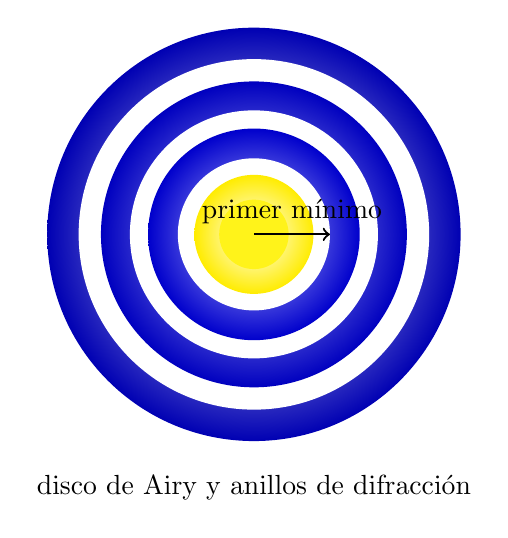
\begin{tikzpicture}[scale=1.05]
  \shade[inner color=white,outer color=blue!70!black] (0,0) circle (2.5);
  \fill[white] (0,0) circle (2.12);
  \shade[inner color=blue!20,outer color=blue!75!black] (0,0) circle (1.85);
  \fill[white] (0,0) circle (1.5);
  \shade[inner color=blue!25,outer color=blue!80!black] (0,0) circle (1.28);
  \fill[white] (0,0) circle (0.92);
  \shade[inner color=white,outer color=yellow!85!orange] (0,0) circle (0.72);
  \fill[yellow!90!white] (0,0) circle (0.42);
  \draw[->,thick] (0,0) -- (0.92,0) node[midway,above] {primer mínimo};
  \node[below] at (0,-2.8) {disco de Airy y anillos de difracción};
\end{tikzpicture}
\caption{Patrón de difracción de una apertura circular.}
\end{figure}